~\vspace{.1in}

\section{Fitting lines to data} 

Thanh has an internship studying road salt usage in a northern metropolitan area.   Road salt is used to melt ice and snow on paved streets.  Because it can damage vegetation and influence both surface water (lakes) and ground water, and because it costs money to run the trucks that apply the salt, people are interested in the amount of road salt used.

One data set compares road salt usage per county.  Thanh learned from county officials  that road salt use varies widely from county to county, but, not surprisingly, it depends heavily on the length of road in the county.
So, the variables are 
\begin{center}
\begin{tabular} {l} 
$L=$ road length (lane miles) $\sim$ indep \\
$S= $ road salt applied (tons per year) $\sim$ dep \\ 
\end{tabular}
\end{center}
A \textbf{lane mile} is the area of road one mile long and one lane wide.  Now you know.

Thanh also learned that while road salt use is a function of lane miles, it is not proportional as there are more complicated factors involved.  Still, he would like to model road salt use as a function of road length.  Here are the data for counties in the metro area.
\begin{center}
\begin{tabular} {|c| |c |c |c |c |c |c |c|}\hline
County & A & C & D & H & R & T & W\\ \hline
$L$ & 710 & 420  & 800 & \text{1,420} & 720 & 510 & 480\\ \hline
$S$ & \text{14,700} & \text{3,900}  & \text{11,600} & \text{15,500} & \text{9,400} & \text{5,000} & \text{9,700} \\ \hline
\end{tabular}
\end{center}
%source: UMN conservancy  Link:  http://conservancy.umn.edu/bitstream/115332/1/pr503.pdf

To develop his model Thanh imagined a new county, County X, that had 600 lane miles of road.  In looking at the data, he finds two counties with close to 600 lane miles.
\begin{center}
\begin{tabular} {|c| |c |c |c|}\hline
& County T & County X &County A \\ \hline
$L$ &  510 & 600 & 710\\ \hline
$S$ &  \text{5,000} & ? & \text{14,700} \\ \hline
\end{tabular}
\end{center}
Based on this data, Thanh expects County X would use between \text{5,000} and \text{14,700} tons/year of road salt.  Since 600 is closer to 510 than to 710, he starts with a guess of around \text{9,000} tons/year of road salt.  

To improve this estimate, Thanh decides to use a linear mode, hoping that will account for both road length influence and fixed factors.  He begins by finding the slope.
 \begin{eqnarray*}
\text{slope} & = & \text{rate of change} = \frac{\text{change dep}}{\text{change indep}} = \frac{\text{14,700}-\text{5,000 tons/year}}{710-510 \text{ lane miles}} \\
& = & (\text{14,700}-\text{5,000})\div(710-510)= 48.5 \text{ tons/year per lane mile}\\
\end{eqnarray*}
%\vspace{-.5in} %VSPACE

\noindent  Next he calculates the intercept.
$$\text{intercept} = \text{dep} -\text{slope}\ast\text{indep}=  \text{5,000} - 48.5\times 510= -\text{19,735 tons/year}$$
He was not expecting a negative value but decides to use it anyway.
Using the template for a linear equation
$$\text{dep} = \text{start} + \text{slope} * \text{indep}$$
Thanh gets
$$S = -\text{19,735} + 48.5L$$
which he rewrites as 
$$S = 48.5L-\text{19,735}$$  % SU this is the TAline
As a check, for $L=710$ lane miles, he gets 
$$S=48.5 \times \underline{710}-\text{19,735}=\text{14,700 tons/year}\quad \checkmark$$  

More importantly, for 600 miles his equation gives the estimate of
$$S=48.5 \times \underline{600}-\text{19,735}=\text{9,365 tons/year}$$  
Thanh rounds this estimate to \text{9,400} tons/year of road salt for County X, which is close to his initial guess of \text{9,000} tons/year.

Next, Thanh imagines another new county, County Y, that has 500 lane miles of road.  He looks to the data for counties with close to 500 lane miles.
\begin{center}
\begin{tabular} {|c| |c |c |c|}\hline
& County W & County Y & County T\\ \hline
$L$ & 480 & 500 & 510 \\ \hline
$S$ & \text{9,700} & ? & \text{5,000} \\ \hline
\end{tabular}
\end{center}
Wait a minute. The county with fewer roads used more salt?  That doesn't make sense.

Thanh decides to look at all the data at once in a scatter plot.
\begin{center}
\scalebox {.8} {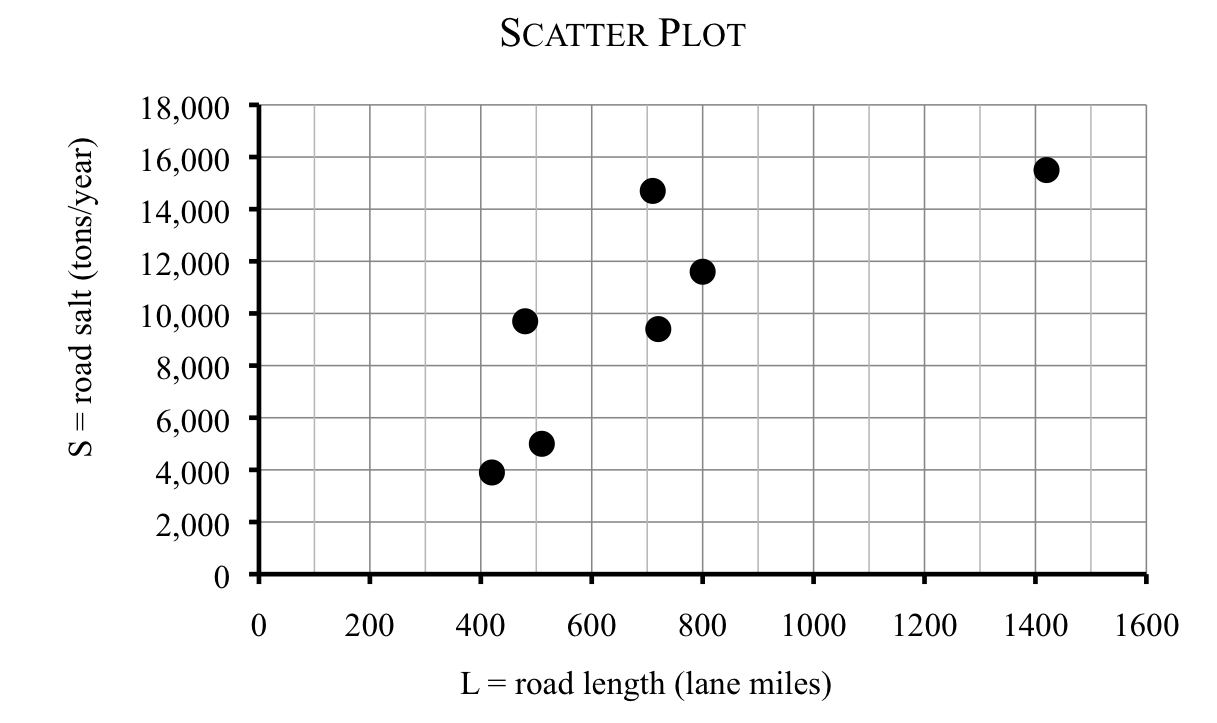
\includegraphics [width = 6in] {roadsaltSCATTER.png}}
\end{center}

\newpage   %%%%%%  NEWPAGE

When Thanh was using the nearby points to estimate for Counties X and Y, it's as if he were connecting the dots with line segments on the graph.  Notice that the line that goes through 500 lane miles is decreasing, just like Thanh saw in his table.
\begin{center}
\scalebox {.8} {\includegraphics [width = 6in] {roadsaltCONNECTDOTS.png}}
\end{center}
 
Thanh suspects that this connect-the-dots model is too heavily influenced by individual county road-salting habits.  He would like a way to get one line to use for everything, knowing full well that one line cannot possibly go through all of the data points.

Which line to use?  One option would be to stick with the line he found through the points for Counties T and A. He redraws the scatter plot to show that line.  Because the intercept is negative, it doesn't show up on his graph. The line seems to be too low at first and too high later.  The problem is that this line is too steep (has too large a slope).
\begin{center}
~\hspace{.35in} \scalebox {.85} {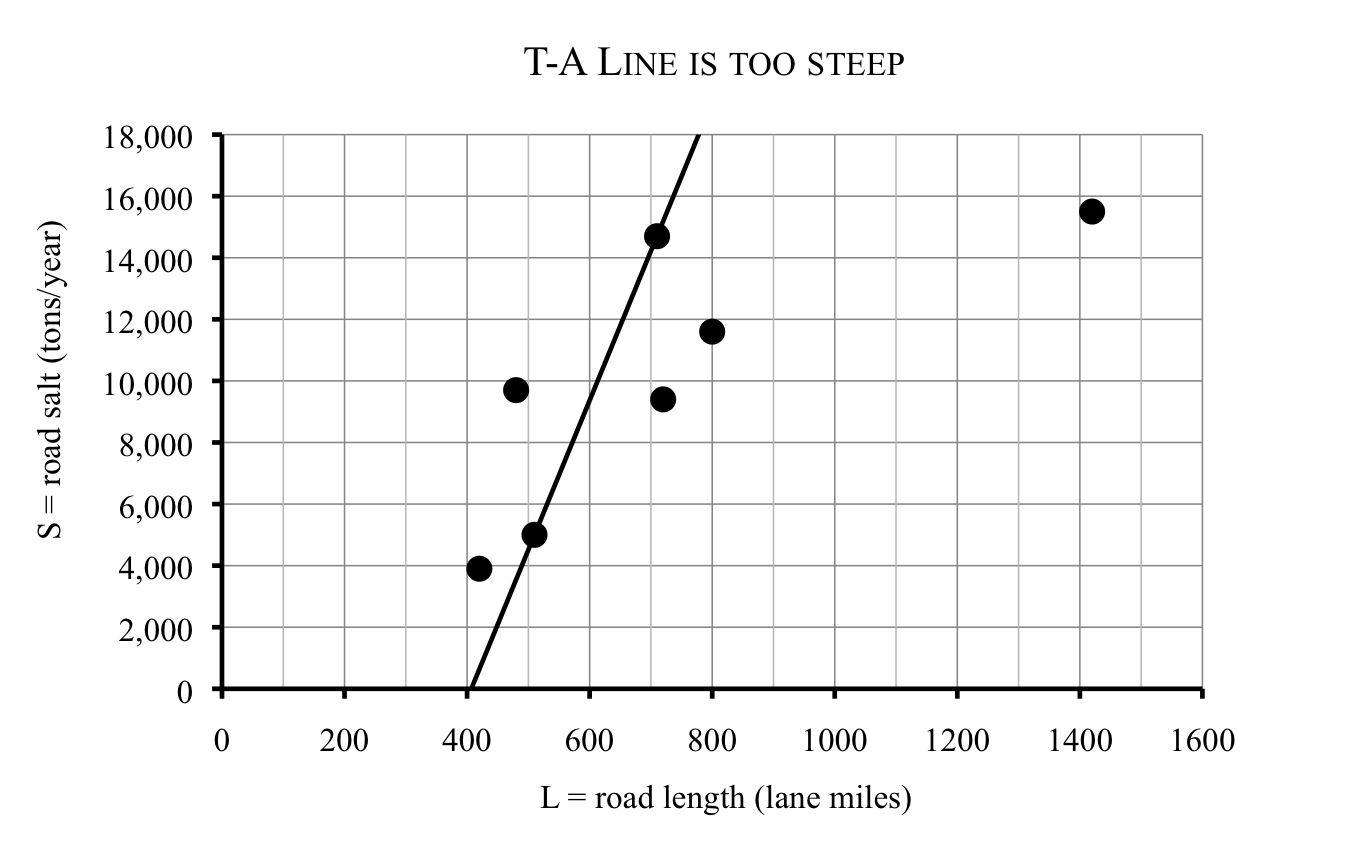
\includegraphics [width = 6in] {roadsaltTAline.png}}
\end{center} %HSPACE

\newpage %%%%%% NEWPAGE

Thanh decides to try a line that is less steep.  After drawing in a few lines, he decides to try the line between the points for Counties C and D instead, which has equation  
$$\textbf{C-D line:} \quad S = 20.26L-\text{4,610}$$
Unfortunately this line seems too low.  (Again the negative intercept isn't visible.)
\begin{center}
\scalebox {.8} {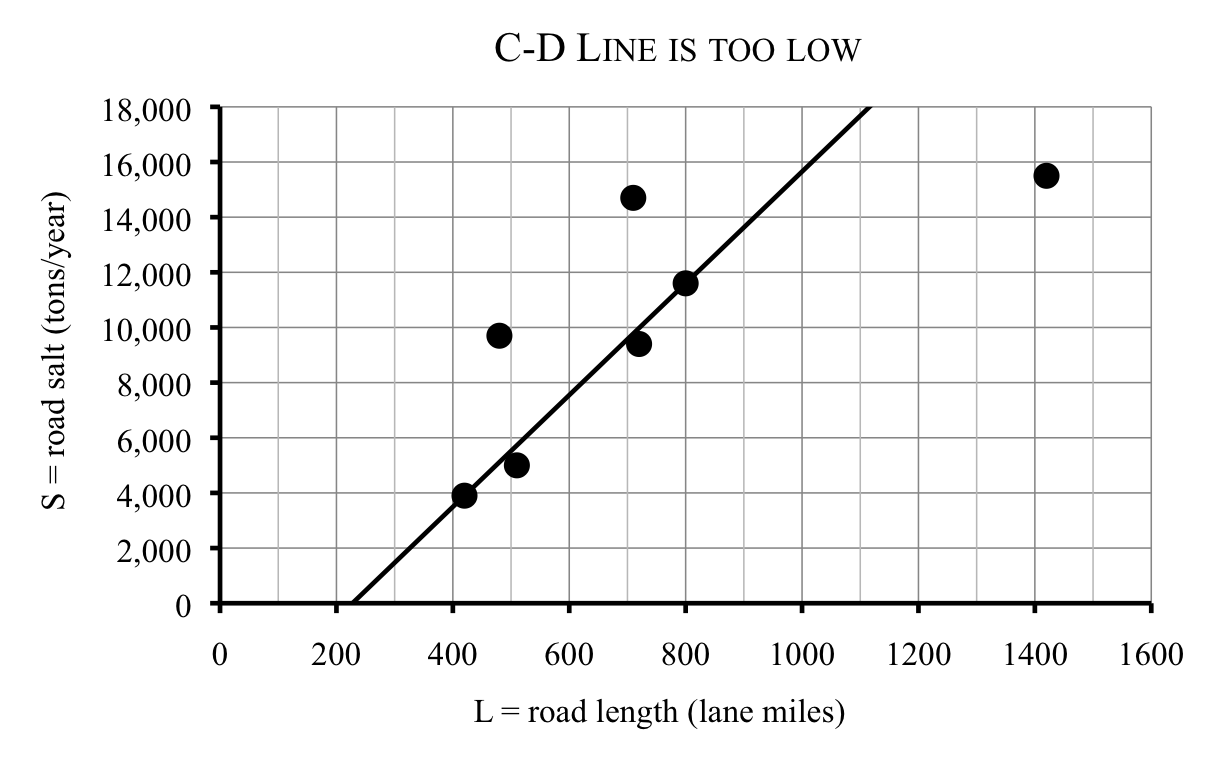
\includegraphics [width = 6in] {roadsaltCDline.png}}
\end{center}

Neither of these lines came close to the point for County H on the far right, so Thanh considers one more line, this time through County H and County R, which has equation 
$$\textbf{H-R line:} \quad S = 8.71L+\text{3,130}$$
This line has a positive intercept just above \text{3,000} tons/year, as you can see on the graph.
\begin{center}
~\hspace{.35in} \scalebox {.87} {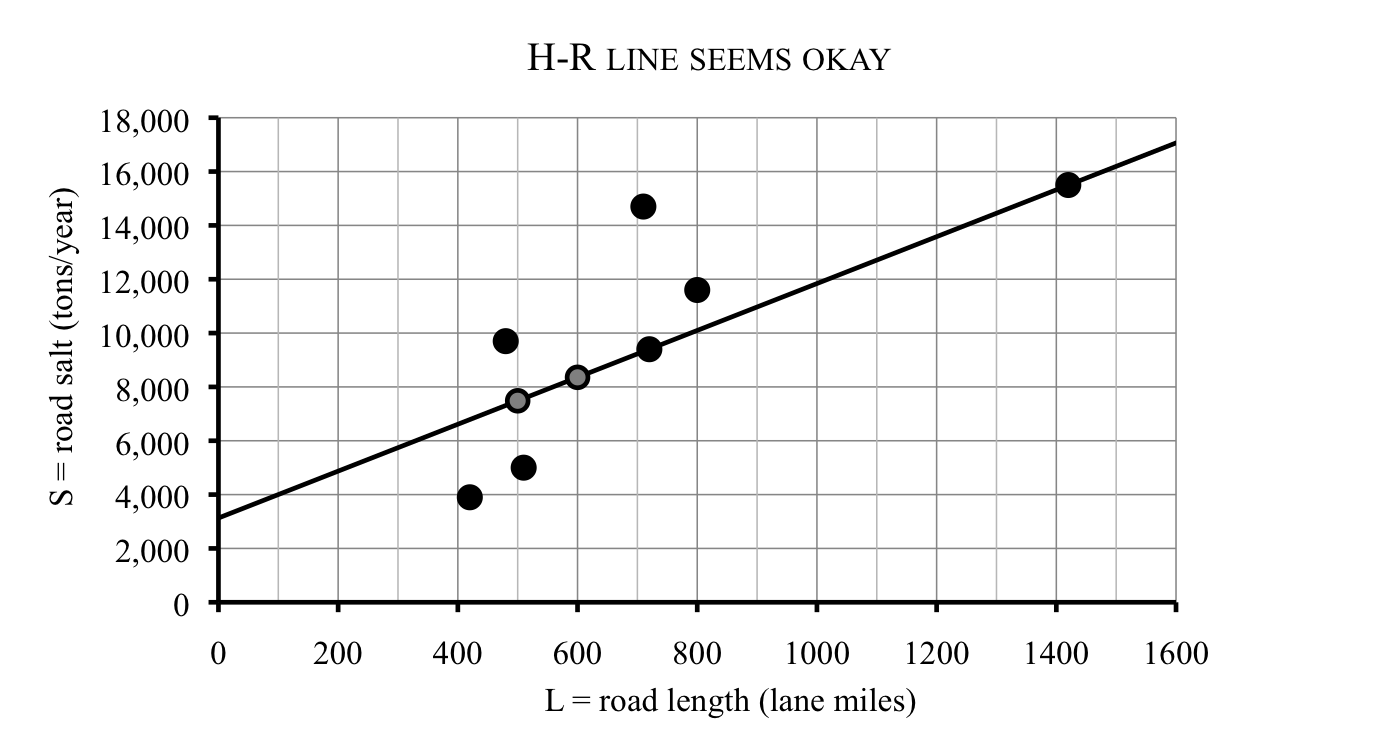
\includegraphics [width = 6in] {roadsaltHRline.png}}
\end{center}  %HSPACE

Thanh thinks the H-R line is reasonable, but it makes him wonder how to decide if one line is better than another.  Generally speaking the \textbf{best fitting line} makes the space between the line and the data points as small as possible.  (There is actually a much more official definition.)  After using a little statistical software, Thanh determines that for this data set, the official best fitting line has equation 
$$\textbf{Best fitting line:} \quad S = 10.0L+\text{2,741}$$

Thanh wants to add this line to his graph so first he calculates a few values.  While it's true that any two points would do, he played it safe and plotted three points, being sure to use 0 in order to find the intercept.
\begin{center}
\begin{tabular} {|c|| c| c| c|}\hline
$L$ &  0 & 600 & \text{1,500} \\ \hline
$S$ & \text{2,741} & \text{8,741} & \text{17,741} \\ \hline
\end{tabular}
\end{center}
He graphs this line and notices it is very similar to the H-R line, just a tiny bit higher and a tiny bit steeper.  The points from the table are highlighted on the graph just to help you see how we graphed the line.  Remember, those aren't actual data points.
\begin{center}
\scalebox {.8} {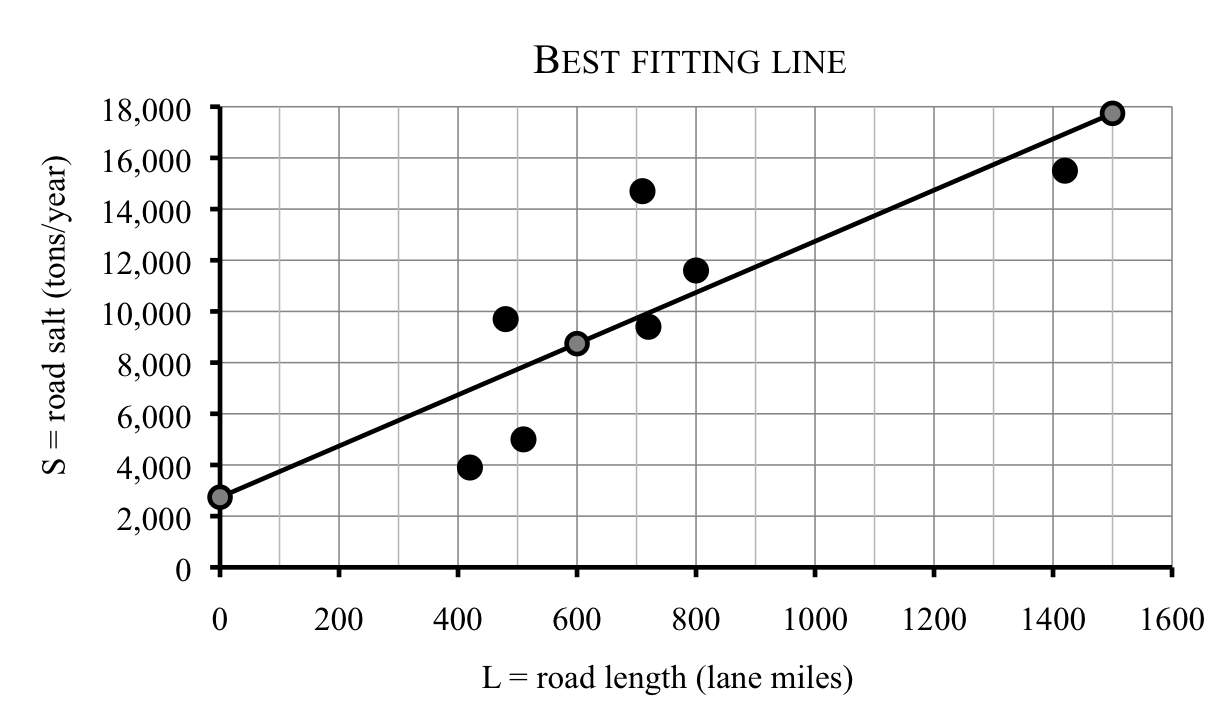
\includegraphics [width = 6in] {roadsaltbestfit.png}}
\end{center}

Thanh is bothered by the fact that County H  seems to be off on its own.  The largest city in this area is in County H.   Between the budget crunch and the nature of the urban landscape, the city tends to use much less road salt than the surrounding areas.  So County H really isn't very typical at all.  In statistics, this sort of value is known by the descriptive term \textbf{outlier} (as in ``it lies way out there.'')

So Thanh decides to look at the statistically best-fitting line ignoring County H this time.  Back to his software and he finds
$$\textbf{Best fitting line (ignoring outlier):} \quad S = 19.7L-\text{2,905}$$
This line is less steep than the T-A line and higher than the C-D line.  Seems perfect.
\begin{center}
\scalebox {.8} {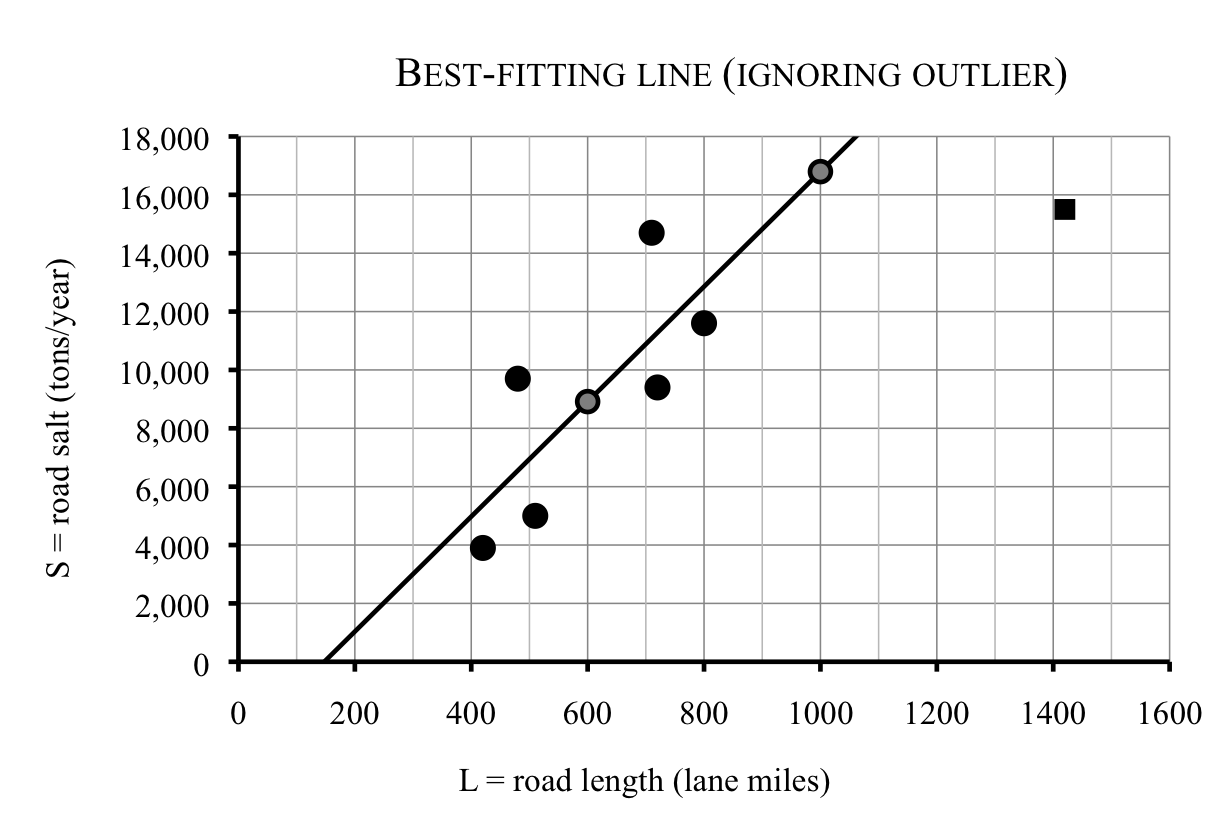
\includegraphics [width = 6in] {roadsaltbestfitwoOutlier.png}}
\end{center}


 %\section{Fitting lines to data}

\begin{center}
\line(1,0){300} %\line(1,0){250}
\end{center}

\section*{Homework}

\noindent \textbf{Start by doing Practice exercises \#1-4 in the workbook.}

\bigskip

\noindent \textbf{Do you know \ldots}

\begin{itemize} 
\item What a scatter plot is? 
\item Why we might begin the scale for a scatter plot somewhere other than 0?
\item Why we would approximate data with a linear function? 
\item How to decide visually whether a line is a reasonable approximation of the data? 
\item The name for a point that falls very far away from an approximating line? 
\item How to graph a line from its equation by creating a table first.
\item Why even the best fitting line doesn't go through most of the data points?
 \item[~] \textbf{If you're not sure, work the rest of exercises and then return to these questions.  Or, ask your instructor or a classmate for help.}   
\end{itemize}

\subsection*{Exercises}

\begin{enumerate} 
\setcounter{enumi}{4}

\item Look back at Thanh's data in the section.
\begin{enumerate}
\item Check that the C-D line has equation $S=20.26L-4,610$
\item Check that the H-R line has equation $S=8.71L+3,130$
\item The best-fitting line (ignoring the outlier) had equation $S = 19.7L-2,905$.  Make a table of values for $L=600$ and $1,000$ lane miles and use these values to check the graph Thanh drew.  (They are highlighted on the graph.)
\end{enumerate}

\item Wild rice is a native plant that grows in lakes in the upper Midwest.  The table shows how the annual acreage of wild rice has varied with the average spring temperature in various years.  The variables are $T$ for the temperature measured in $^{\circ}$F and $W$ for the wild rice yield, measured in acres.  In case you're curious, the year is included as well, but it's not one of the variables we're interested in.
\begin{center}
\begin{tabular} {|c||c|c |c|c|c|c|c|}  \hline
year & 1985 & 1989 & 1993 & 1997 & 2001 & 2005 & 2009  \\ \hline
$T$ & 39 & 42 & 41 & 35 & 47 & 45 & 42
 \\ \hline
$W$& 2,300 & 1,950 & 1,425 & 2,015 & 1,233 & 1,256 & 1,345 \\ \hline
\end{tabular}
\end{center}
\hfill \emph{Story also appears in 4.1 Exercises}
\begin{enumerate}
\item Make a scatter plot of the points.  Make your graph as large as possible by starting your temperature axis at 35$^{\circ}$F and your acreage axis at 1,000 acres.
\item Find the equation of the line through the data from 1997 and 2001. Use $T$ for the average temperature (in $^{\circ}$F) and $W$ for the acres of wild rice.
\item Based on your line, what might you expect the acreage of wild rice to be in a year when the average temperature is 46$^{\circ}$F?  40$^{\circ}$F?  Use your equation to answer the questions.
\item Draw that line on your scatter plot.  Comment.
\item The best fitting line has equation $$W=5,072.2-82.41T$$  Make a table of values and use it to graph that line as well.
\item If you use the best fitting line, how would that change your estimate for the acreage of wild rice in a year when the average temperature is 46$^{\circ}$F?  40$^{\circ}$F?  
\end{enumerate} % DATA is in Excel file: wildrice.xlsx

\item The amount of garbage generated in the United States has increased steadily, from 88.1 million tons in 1960 to 254.2 million tons in 2006. Earlier we did linear model. 
But, in fact, the amount of garbage has not increased exactly linearly.  The table shows data for select years, where $Y$ measures years since 1960 and $G$ is the amount of garbage (in millions of tons).
\begin{center}
\begin{tabular} {|c||c|c |c|c|c|c|c|c|c|}  \hline
year & 1960 & 1970 & 1980 & 1990 & 2000 & 2006 & 2010 \\ \hline
$Y$ & 0 & 10 & 20 & 30 & 40 & 46 & 50 \\ \hline
$G$ & 88.1 & 121.1 & 151.6 & 205.2 & 239.1 & 254.2 & 249.0 \\ \hline
\end{tabular}
\end{center}
\hfill \begin{footnotesize} Source:  Environmental Protection Agency \end{footnotesize}

\hfill \emph{Story also appears in 4.4 Exercises.}

\begin{enumerate}
\item Make a large scatter plot of the points, beginning at the year 1960 and extending to at least 2030.  
\item Draw in the line through the points from 1960 and 2006.  (We found that equation in 4.4 Exercises.)  
\item Draw in the line through the points from 2000 and 2006.  Would this line predict that garbage will reach 300 million tons sooner or later than the previous prediction?  Use the graph to explain. 
\end{enumerate}  

\item My mechanic, Paye, believes that frequent oil changes reduce the amount of maintenance on a car.  To prove his point, Paye showed me a table of customers with the number of yearly oil changes and the cost of their engine repairs. 
\begin{center} 
\begin{tabular} {|c||c|c |c|c|c|c|c|}  \hline
$N$& 1 & 2 & 3 & 4 & 5 & 6 & 7  \\ \hline
$R$& 725 & 500 & 415 & 300 & 275 & 100 & 150  \\ \hline
\end{tabular}
\end{center}
where $N$ is the number of oil changes per year and $R$ is the cost of repairs, in dollars.
\begin{enumerate}
\item Make a large scatter plot of the points. 
\item Draw in the line through the points for 3 and 5 oil changes.  
\item Write the equation for that line.  Use your equation to predict the cost of engine repairs for a customer who does no oil changes, and one who does 8 oil changes.
\item The best fitting line has equation approximately $$R=732.86-95.179N$$
Plot three points on that line and use them to draw it on your scatter plot.
\item What does the best fitting line predict the cost of engine repairs for a customer who does no oil changes, and one who does 8 oil changes?
\end{enumerate}  % DATA is in Excel file:  oilchanges.xlsx

\item The table and scatterplot shows the estimated costs and earnings for various sports-themed movies.
\begin{center}
\begin{tabular} {|l|r|r|} \hline
Movie & Estimated cost & Estimated earnings \\ \hline  \hline
A League of Their Own & \$40 million & \$131 million \\ \hline
Dodgeball & \$30 million & \$114 million \\ \hline
Invictus & \$49 million & \$37 million \\ \hline
Jerry Maguire & \$60 million & \$274 million \\ \hline
Miracle & \$28 million & \$64 million \\ \hline
%Moneyball & \$50 million & \$75 million \\ \hline
Nacho Libre & \$32 million & \$80 million \\ \hline
Remember the Titans & \$27 million & \$130 million \\ \hline
Run Fatboy Run & \$10 million & \$6 million \\ \hline
%Seabiscuit & \$86 million & \$120 million \\ \hline
Secretariat & \$35 million & \$59 million \\ \hline
The Blind Side & \$35 million & \$255 million \\ \hline
The Rookie & \$22 million & \$77 million \\ \hline
\end{tabular}
\end{center}
\begin{center}
\scalebox {.8} {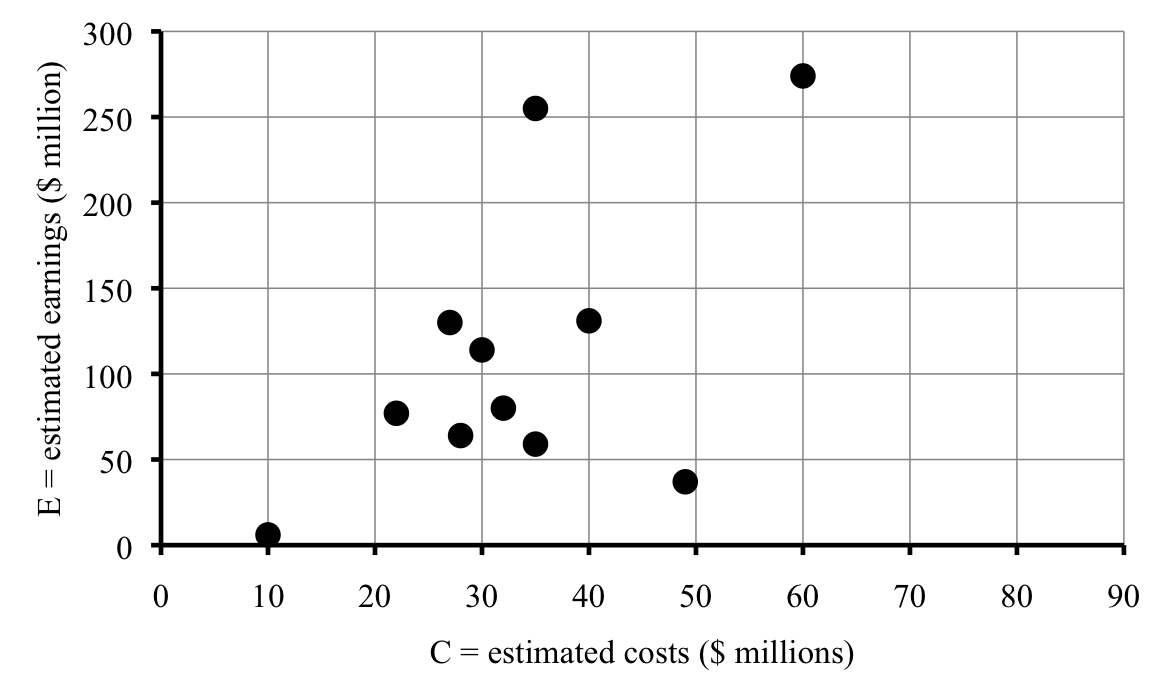
\includegraphics [width = 6in] {sportsmovies.png}}
\end{center}
\begin{enumerate}
\item Draw the line (A)  that goes through the points for ``Remember the Titans'' and ``A League of Their Own''.  Explain why this line does not fit the data well.  
\item Draw the line (B) that goes through the points for ``Run Fatboy Run'' and ``Jerry Maguire''. Explain why this line does not fit the data well.
 \item Draw the line (C) that goes through the points for ``The Rookie'' and ``A League of Their Own''.  This line fits the data pretty well I think.
\item Why might you expect the slope of good fitting line to be positive?
\end{enumerate} % source: Good wikipedia page for listing of sports movies: http://en.wikipedia.org/wiki/List_of_sports_films Website for box office numbers: http://www.the-numbers.com/
% DATA is in Excel file sportsmovies.xlsx

\item The annual consumption of meat in millions of metric tons is given in the following table. Here $C$ is for chicken, $B$ is for beef, and $Y$ measures years since 1975.

\hfill \begin{footnotesize} Source: U.S. Department of Agriculture \end{footnotesize}
\begin{center}
\begin{tabular} {|c| |c |c |c |c |c |c |c |c |c |c|}\hline
year & 1975 & 1985 & 1990 & 1995 & 2000 & 2005 & 2009 & 2012\\ \hline
$Y$ & 0 & 10 & 15 & 20 & 25 & 30 & 34 & 37\\ \hline
$C$ & 3.6 & 6.1 & 7.7 &9.4 & 11.5 & 13.4 & 12.9 & 13.3\\ \hline
$B$ & 12.1 & 11.8 & 11.0 & 11.7 & 12.5 & 12.7 & 12.2 & 11.4\\ \hline
\end{tabular}
\end{center}
\begin{enumerate}
\item Make a scatter plot of the chicken consumption (use $\ast$ to label each point) and red meat consumption (use $\circ$ to label each point).
\item Sketch a line through each data set that seems to reasonably approximate the dependence.
\item When were chicken and red meat consumption equal?
\item The best fitting line for chicken is $$C =3.6375+0.2854Y$$ and the best fitting line for beef is $$B=11.774+0.007Y$$  Set up and solve a system of linear equations to find the year when  chicken and red meat consumption will likely be equal.  How does this answer compare to your estimate?
\item The slope of the best fitting beef line is 0.007 million tons/year. What does that tell you about beef consumption over the past 40 years?
\end{enumerate}  %Go to: http://www.earth-policy.org/data_center/C24  search for meat consumption to get excel spreadsheet of values collated from USDA http://www.freakonomics.com/2010/12/09/beef-or-chicken-a-look-at-u-s-meat-trends-in-the-last-century
% DATA is in Excel file chickenorbeef?.xlsx

\end{enumerate}
